\section{Approach}
\label{sec:approach}

\begin{figure*}[t!]
    \centering
    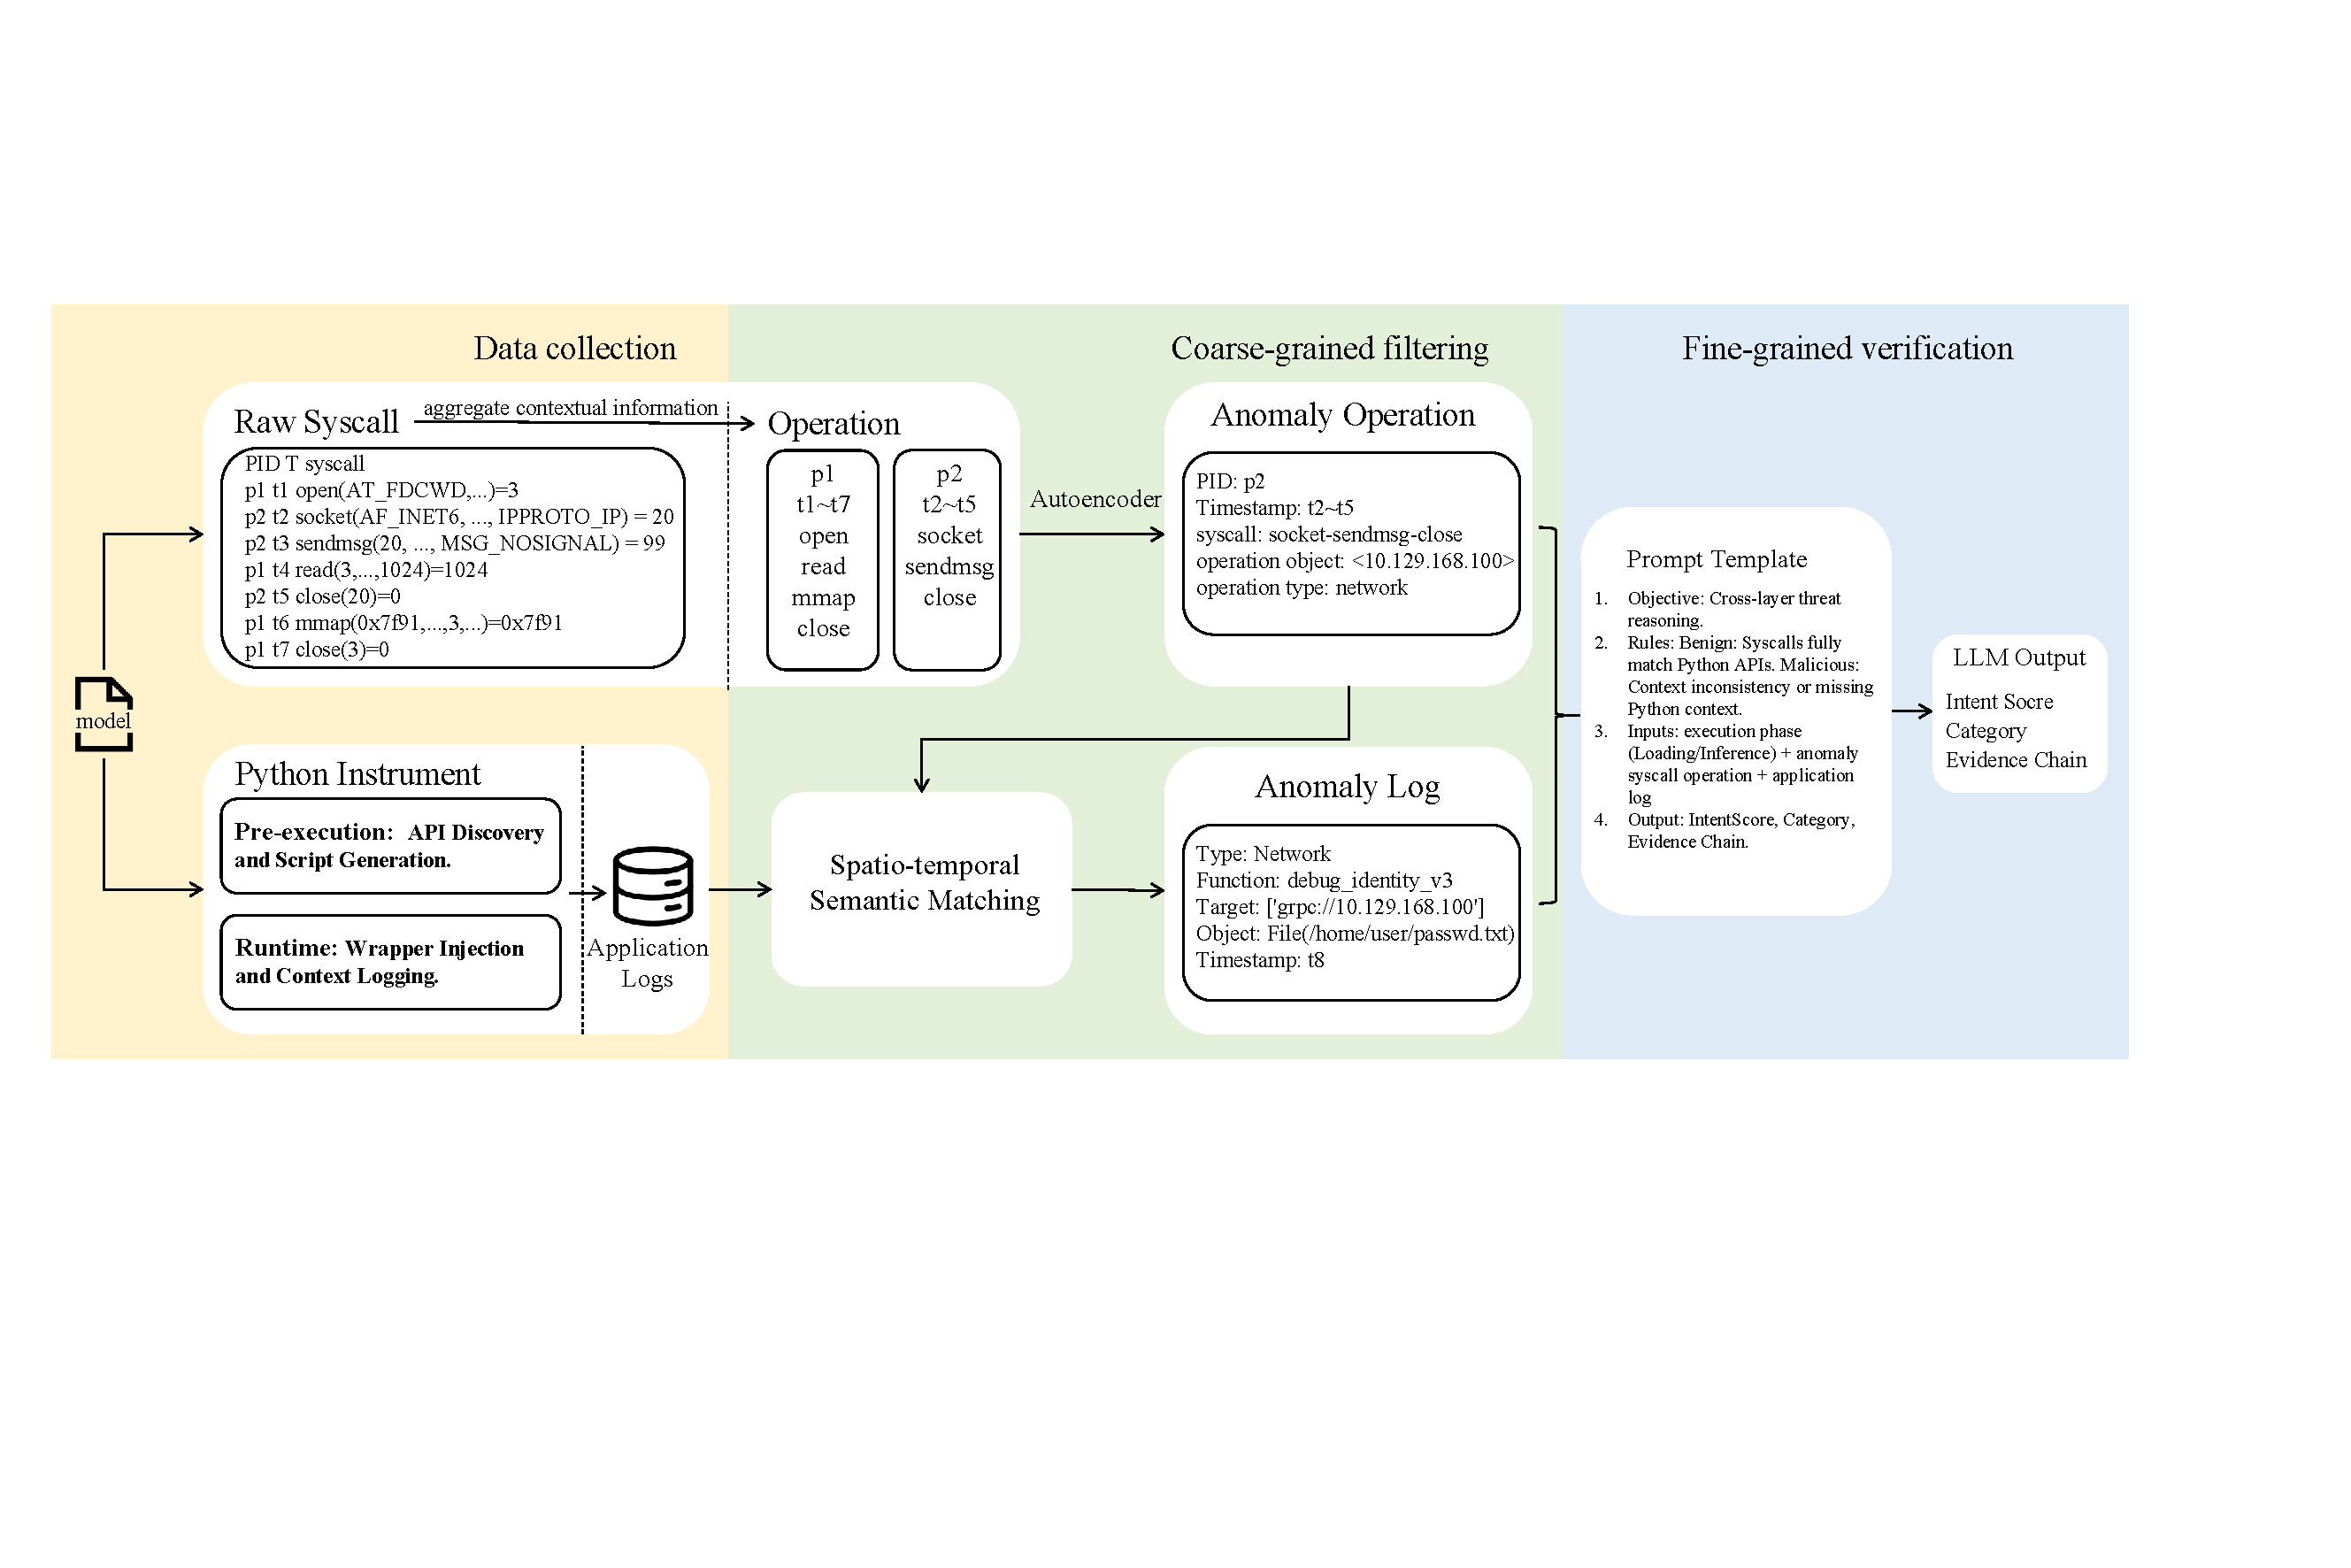
\includegraphics[width=\linewidth]{figs/overview4.pdf}
    \caption{Overview of the hybrid defense system.}
    \label{fig:overview}
\end{figure*}


In this section, we present our approach for detecting malicious behaviors embedded in model artifacts. The pipeline operates in three stages: (i) \emph{Data Collection}, which gathers two synchronized evidence streams, low-level system-call traces and high-level Python semantic logs; (ii) \emph{Coarse-grained Filtering}, which clusters raw system calls into operation vectors, screens for anomalies via an unsupervised autoencoder, and retrieves aligned semantic context through fuzzy spatio-temporal matching; and (iii) \emph{Fine-grained Verification}, where an LLM jointly reasons about the system-call evidence and Python semantic context to produce an intent score, a threat category, and an auditable evidence chain.

\subsection{Data Collection}

The data collection stage simultaneously captures two synchronized streams of evidence during controlled model execution: a kernel-visible system-call stream and an application-layer semantic log stream. Together, these streams provide the complementary low-level and high-level signals needed for downstream analysis.

\subsubsection{System-call collection.}
We base our detection on system-call traces because they operate below the user-space level and cannot be bypassed by any Python-level obfuscation~\cite{2875487}: no matter how a model artifact hides its malicious intent through code mangling or dynamic loading, its actual interactions with the operating system must traverse the kernel and therefore leave a non-bypassable forensic record.

\begin{table}[t!]
	\centering
	\caption{Security-relevant system-call categories used by our filter.}
	\begin{tabular}{p{0.10\columnwidth} p{0.28\columnwidth} p{0.47\columnwidth}}
		\hline
		Param & Category & Purpose \\
		\hline
		file   & File operations  & Detect sensitive data leakage or configuration file tampering \\
		network & Network operations  & Detect data exfiltration or remote command execution \\
		cred   & Credential operations  & Detect privilege-escalation behavior \\
		desc   & Descriptor operations  & Detect file-related malicious behavior detection \\
		signal & Signal handling  & Capture malicious process termination attempts \\
		clock  & Time-related operations & Assist temporal anomaly analysis  \\
		\hline
	\end{tabular}
	\label{tab:syscalltypes}
\end{table}

We employ a selective tracing strategy that focuses exclusively on security-relevant system-call families, discarding high-frequency but semantically uninformative calls to keep the trace volume manageable. During controlled model execution, we use \texttt{strace} to continuously trace system calls of the target process. To reduce noise and overhead, we immediately discard calls such as scheduler hints and memory-mapping operations that carry no security signal\cite{shakya2022analysisdetectionclassificationandroid}. Table~\ref{tab:syscalltypes} summarizes the security-relevant syscall families we monitor and their roles in our detection pipeline. For example, file operations can reveal attempts to access sensitive data or modify configurations, while network operations may signal data exfiltration or remote command execution.

\subsubsection{Instrumentation log collection.}
To bridge the semantic gap between model-level intent and kernel-level behavior, we collect high-dimensional Python semantic context via non-invasive instrumentation. The key challenge is that heterogeneous ML frameworks expose frequently changing APIs, making manual per-framework instrumentation labor-intensive and coverage-incomplete. We address this through an LLM-assisted approach with two distinct phases.

\noindent \textbf{Pre-execution: API discovery and script generation.}
Before model execution, we first determine which modules to instrument by automatically discovering the model's import dependencies. We analyze the model's loading entry point and the packages it imports—covering both ML frameworks and standard-library modules that deserialization-based attacks rely on. So that instrumentation coverage follows each model's actual dependency surface rather than a fixed, pre-defined module list. For each discovered module $\mathcal{M}$, we then leverage an LLM to synthesize a dynamic instrumentation script. A rigorously structured prompt constrains the LLM to generate code that inspects $\mathcal{M}$'s namespace at startup, systematically identifies all public callable attributes, and constructs wrapper closures around each. The prompt specifies the security objective, mandates capturing execution context which contains timestamps, operation types, argument values and return types, and requires all intercepted events to be serialized into standardized JSON. This automated discovery eliminates statically hardcoded API lists and adapts to framework version changes by simply regenerating wrappers for the new API surface, without modifying the core detection pipeline. Our instrumentation intercepts all public callables of the target library, wraps only callable functions, and serializes arguments defensively, so it is neither a whitelist nor a blacklist. The prompt fixes a deterministic skeleton that works across frameworks, and the LLM rebuilds framework-specific security semantics on demand, which is what lets coverage track framework API evolution without manual per-framework coding.

Algorithm~\ref{alg:instrumentation} formalizes this discovery and wrapping logic. The \texttt{ApplyDynamicPatches} procedure is invoked once per discovered module $\mathcal{M}$; it isolates public callables while skipping private attributes and non-callable objects, then generates wrapper closures for each target API.

\begin{algorithm}[t!]
\caption{Automated Dynamic Instrumentation Logic}
\label{alg:instrumentation}
\KwIn{Target module $\mathcal{M}$ discovered from the model's imports}
\KwOut{Instrumented module capable of context logging}

\SetKwProg{Fn}{Procedure}{:}{}
\SetKwFunction{FApply}{ApplyDynamicPatches}
\SetKwFunction{FConstruct}{Wrapper}

\Fn{\FApply{$\mathcal{M}$}}{
    \ForEach{attribute name $attr\_name$ \textnormal{\textbf{in}} \textnormal{dir}($\mathcal{M}$)}{
        \If{$attr\_name$ starts with ``\_''}{
            \textbf{continue} 
        }
        
        $target\_func \gets$ \textnormal{getattr}($\mathcal{M}, attr\_name$)\;
        \If{\textnormal{\textbf{not}} is\_callable($target\_func$)}{
            \textbf{continue} 
        }
        
        $wrapper \gets$ \FConstruct{$target\_func, attr\_name$}\;
        
        \textbf{try}\;
        \Indp \textnormal{setattr}($\mathcal{M}, attr\_name, wrapper$)\; 
        \Indm \textbf{catch} \textit{ReadOnlyAttributeError} \;
        \Indp \textbf{continue} \;
        \Indm
    }
}
\Fn{\FConstruct{$func, name$}}{
    \KwRet a closure that captures the full \texttt{traceback}, logs to JSON, executes $func$, and delegates return value\;
}
\end{algorithm}

\noindent \textbf{Runtime: wrapper injection and context logging.}
At process startup, the generated script employs monkey patching (\texttt{setattr}) to replace original functions with wrapper closures. Thereafter, any invocation of a wrapped API triggers the injected closure, which captures the execution context and serializes it as a structured semantic event:
\begin{equation}
\ell_i = \langle \textit{FuncName},\; \textit{ArgsSummary} \rangle.
\end{equation}
Here $\textit{FuncName}$ denotes the invoked framework or standard-library API, while $\textit{ArgsSummary}$ aggregates only lightweight information—tensor shapes and dtypes, configuration flags, truncated or hashed file paths, and bounded-length string summaries—controlling logging overhead while preserving rich contextual signals.

To ensure runtime safety, wrappers follow a conservative policy: they only wrap callable functions avoiding class definitions, built-in types, and C/C++ bindings, perform best-effort argument summarization without altering return values or side effects, and employ defensive serialization. The patching process is additionally wrapped in \texttt{try-except} blocks to survive read-only properties, immutable C-extension bindings, and dynamically generated descriptors that would otherwise crash the process. Any patch failure degrades gracefully without disrupting the target process.

\subsection{Coarse-grained Filtering}

After collecting raw evidence streams, the coarse-grained filtering stage transforms system-call traces into compact operation vectors, screens for anomalies, and retrieves the corresponding semantic context. This stage eliminates clearly benign activity before the expensive LLM reasoning stage.

\subsubsection{System-call Clustering and Embedding}

The collected system-call traces are extremely fine-grained and voluminous. A single model loading process may produce thousands of system calls, and meaningful malicious behavior invariably manifests as a sequence of related calls rather than as isolated events. To address this, we aggregate correlated system calls into compact high-level operation vectors to reduce trace noise and compress data volume, while providing standardized analysis units with complete semantics for anomaly detection.

To accurately model the execution semantics of a program, it is crucial to recognize that system calls inherently possess varying degrees of contextual dependency. Applying a uniform extraction strategy to all system calls would be ineffective: some operations are semantically self-contained and immediately indicative of high-risk behavior, whereas others are granular, stateful operations that remain ambiguous unless analyzed as a continuous sequence. Motivated by this fundamental difference, we propose a hybrid embedding scheme that categorizes the traced system calls into two distinct streams for targeted handling: (1) \emph{Directly malicious calls} and (2) \emph{Stateful calls}. By processing these two streams individually, we ultimately synthesize them into a unified feature space for downstream analysis.

\noindent \textbf{Direct call embedding.}
The first category includes standalone, high-risk operations that do not require lifecycle context. We encode each such call into a vector $\mathbf{v}_{\textit{dir}} \in \mathbb{R}^{d}$ with $d=128$. We use a custom small BERT derived from \texttt{bert-base-uncased}. The weights are continued from the \texttt{bert-base-uncased} checkpoint rather than randomly initialized, so the model retains its pre-trained language understanding. The input text for a syscall is its serialized form \texttt{syscall(args)}. We further pretrain this BERT on the strace logs of the benign training models with masked language modeling and next-sentence prediction, where each log line is one complete syscall record: a positive NSP pair  consists of two adjacent lines $(i,\, i{+}1)$, and a negative pair pairs line $i$ with a randomly sampled line more than five positions away. The 128-dimensional \texttt{[CLS]} vector of the resulting model serves as $\mathbf{v}_{\textit{dir}}$.

\noindent \textbf{Stateful aggregation.}
Stateful operations are grouped by the file or socket descriptor they operate on, rather than analyzed call by call. As the trace is streamed, we buffer every event whose syscall targets a given descriptor \textit{FD} into a per-\textit{FD} list, starting from the resource-acquisition call (e.g., \texttt{open} or \texttt{socket}) and ending at the matching release call (e.g., \texttt{close} or \texttt{shutdown}). When the release call is observed, the entire buffered list is popped as one ordered sequence $S_r = (e_1, \dots, e_{n})$ that captures the full lifetime of that file handle or connection. Each event $e_k$ in the sequence is then serialized into the same \texttt{syscall(args)} text form used for direct calls and independently encoded by the BERT embedding model, yielding a 128-dimensional vector $\mathbf{b}_k = \text{BERT}(\textit{syscall}_k(\textit{args}_k))$ per event. Stacking these gives the stateful operation representation
\begin{equation}
\mathbf{v}_{\textit{sys}}(r) = \big[\,\mathbf{b}_1,\; \mathbf{b}_2,\; \dots,\; \mathbf{b}_{n}\,\big] \in \mathbb{R}^{n \times 128},
\end{equation}
a variable-length $(\textit{seq\_len}, 128)$ sequence rather than a single fixed-length vector. This design reuses the same BERT that encodes direct calls, so both streams share a common per-syscall semantic space, while the stateful stream additionally preserves the order and co-occurrence of calls within each resource lifecycle. The resulting sequence is consumed directly by the LSTM-based SeqAE described next, which handles the variable length $n$ natively.

Rather than merging the two streams into a single representation, we keep $\mathbf{v}_{\textit{dir}}$ and $\mathbf{v}_{\textit{sys}}$ separate and route each to a dedicated anomaly detector. A single syscall and a resource lifecycle segment have fundamentally different shapes and forcing them into one reconstruction model would distort both. Directly malicious calls are thus screened for immediate, self-contained threats, while stateful segments are analyzed in context for subtler malicious behavior.

\subsubsection{Autoencoder-based Anomaly Detection}

We adopt unsupervised anomaly detection because benign model loading and inference produce a stable, learnable distribution of system-call operations, whereas malicious behaviors are inherently rare and diverse, making supervised classification impractical without labeled attack samples that cover the full threat space. Among unsupervised methods, we choose Autoencoders for their conceptual simplicity and proven effectiveness in reconstruction-based anomaly detection: each learns to faithfully reconstruct one type of benign operation vector during training and naturally flags any vector it cannot faithfully reconstruct as anomalous.

Because the two embedding streams have different shapes, we train two independent autoencoders rather than a single shared one. A \textbf{DirectAE}, an MLP-based autoencoder, reconstructs the 128-dimensional single-syscall embedding $\mathbf{v}_{\textit{dir}}$; a \textbf{SeqAE}, an LSTM-based autoencoder, reconstructs the $(\textit{seq\_len}, 128)$ sequence embedding $\mathbf{v}_{\textit{sys}}(r)$ of each resource lifecycle segment. Each is trained on the corresponding operation vectors collected from benign execution, using strace traces of ten benign Hugging Face models (bert-base-uncased, MiniLM-L6-H384-uncased, bert-base-chinese, distilgpt2, t5-small, resnet-50, emotion-english-distilroberta-base, whisper-tiny, twitter-roberta-base-sentiment, and tapas-base-finetuned-wtq), each loaded once with one typical inference, and both are optimized with MSE reconstruction loss.

The two autoencoders maintain independent reconstruction thresholds each set at the 99.9th percentile of the reconstruction error on its own benign training set. Given an operation vector $\mathbf{v}$, the matching autoencoder computes a reconstruction error
\begin{equation}
E = \left\lVert \mathbf{v} - \textit{Dec}(\textit{Enc}(\mathbf{v})) \right\rVert_2^2,
\end{equation}
where \textit{Enc} and \textit{Dec} denote the encoder and decoder of the corresponding autoencoder. An operation is flagged as abnormal if its error exceeds its stream's threshold; otherwise it is discarded as consistent with normal behavior. The abnormal operations from both streams are then unified and promoted to the spatio-temporal matching stage, each carrying its full underlying system-call segment $S'$ and metadata $\langle \textit{PID}, \textit{TID}, t_{\textit{start}}, t_{\textit{end}} \rangle$ for downstream cross-layer association and LLM verification.

By performing this unsupervised prefiltering at the operation level, the system keeps the expensive cross-layer association and LLM reasoning off the critical path for the vast majority of benign activity, while still surfacing rare, suspicious low-level behaviors that deviate from the learned distribution of normal AI model execution.

\subsubsection{Spatio-temporal Semantic Matching}

After the autoencoder identifies abnormal operations, we must determine whether each anomaly can be explained by benign Python-level behavior. This requires retrieving the semantic context from the instrumentation log stream that corresponds to each abnormal system-call operation. However, naive one-to-one timestamp matching between system-call logs and semantic logs is unreliable in high-concurrency workloads. We therefore adopt a fuzzy spatio-temporal association strategy.

For each abnormal operation, the autoencoder screening stage provides the underlying system-call segment $S'$ and its metadata $\langle \textit{PID}, t_{\textit{start}}, t_{\textit{end}} \rangle$. Given this metadata and the semantic log stream $L = \{(\ell_i, t_i)\}$, we perform filtering following the spatial-temporal matching rules below.

\noindent \textbf{Temporal windowing.}
We apply a slack temporal window around the abnormal operation. For each candidate abnormal operation, we define its active time span $[t_{\textit{start}}, t_{\textit{end}}]$ based on the first and last system call in $S'$, and search semantic events whose timestamps $t_i$ fall into an expanded window $[t_{\textit{start}} - \Delta t, t_{\textit{end}} + \Delta t]$. The slack parameter $\Delta t$ tolerates minor scheduling jitter while still localizing semantic context to the period when the resource was actually in use.

\noindent \textbf{Spatial hints.}
Temporal proximity alone is insufficient under heavy concurrency. We therefore further filter candidates using resource-related hints derived from both layers, such as whether the operation is file- or network-related, file paths or prefixes, remote destinations, and other descriptor metadata when available. Combining temporal and spatial constraints yields a fuzzy but robust alignment that significantly reduces spurious associations when many model components execute in parallel.

\subsection{Fine-grained Verification}

Operations that survive coarse-grained filtering are escalated to the fine-grained verification stage, which jointly reasons about the low-level system-call evidence and high-level semantic context to produce a final intent judgment.

Determining whether abnormal low-level operations reflect benign model behavior or malicious intent is inherently challenging: the same system-call pattern can arise from legitimate model loading or from an attacker's attempt to exfiltrate data, and without semantic context the two are indistinguishable at the kernel level. To resolve this ambiguity, we feed each abnormal operation together with its aligned semantic contexts into an LLM, which judges whether the behavior is consistent with benign model execution. We use deepseek-v4-pro for cross-layer reasoning with temperature=0 and zero-shot prompting.

\noindent \textbf{Prompt construction.}
We translate the aligned evidence into a structured natural-language prompt that includes: (i) a concise summary of the abnormal operation including operation type, key statistics, and risk-relevant parameters, (ii) the aligned semantic call contexts including library/API, call stack summary, and argument summaries, and (iii) the execution phase categorized into the model loading stage and inference stage.

Our maliciousness judgment follows a principled cross-layer reasoning rule: a behavior is classified as benign only when its low-level system-call activity can be plausibly explained by the aligned Python-level semantic context. Concretely, if the LLM identifies that the observed file reads, network connections, or process creations are consistent with the framework APIs and execution phase reported in the semantic log, the operation is deemed benign and discarded. Conversely, when inconsistencies exist between the Python-layer semantic logs and the corresponding system-call activities, or when no matching Python semantic context can be retrieved at all, the behavior is marked as malicious and escalated. This joint design also lets DDMO resist code-level obfuscation. Such obfuscation can disguise the Python-level semantics that instrumentation records, but it cannot alter the kernel-level system calls the model actually performs. When the code is obfuscated, the instrumentation emits misleading logs or none at all, while the kernel still records the real syscalls, and this misalignment between the two layers is exactly what the joint analysis flags. The TensorAbuse attacks in our dataset rely on this kind of disguise, and DDMO detects them successfully.

\noindent \textbf{Decision and explanation.}
The LLM outputs $\textit{IntentScore}$, a $\textit{ThreatCategory}$ label, and a rationale. Importantly, we persist the subset of semantic events and system-call summaries used in the reasoning as the evidence chain $\textit{Context}$ for auditing.
If high-risk system-call patterns appear without any plausible semantic explanation, the system raises a high-severity alert and can block execution in the controlled environment.


